\documentclass[a4paper]{article}

%% Language and font encodings
\usepackage[spanish]{babel}
\usepackage[utf8x]{inputenc}
\usepackage[T1]{fontenc}

%% Sets page size and margins
\usepackage[a4paper,top=3cm,bottom=2cm,left=3cm,right=3cm,marginparwidth=1.75cm]{geometry}

%% Useful packages
\usepackage[toc,page]{appendix}
\usepackage{listings} % For matlab code
\usepackage{amsmath}
\usepackage{graphicx}
\usepackage{titling}
\usepackage[colorinlistoftodos]{todonotes}
\usepackage[colorlinks=true, allcolors=blue]{hyperref}
\usepackage{color} %red, green, blue, yellow, cyan, magenta, black, white
\definecolor{mygreen}{RGB}{28,172,0} % color values Red, Green, Blue
\definecolor{mylilas}{RGB}{170,55,241}

%% Calc: For picture positioning
\usetikzlibrary{calc}

\pretitle{
\begin{center}
% Udelar - top left
\begin{tikzpicture}[remember picture,overlay]
 \node[anchor=north west,inner sep=0pt] at ($(current page.north west)+(2cm,-2cm)$) {
  
\includegraphics[width=2cm]{assets/udelar_v.png}
 };
\end{tikzpicture}
% Fcien - top right
\begin{tikzpicture}[remember picture,overlay]
 \node[anchor=north east,inner sep=0pt] at ($(current page.north east)+(-2cm,-2cm)$) {
  
\includegraphics[width=2cm]{assets/fcien_v.png}
 };
\end{tikzpicture}
}
\posttitle{\end{center}}

\title{\large Introducción a las Ciencias de la Tierra y el Espacio I\\[0.5cm]
Práctica 2\\[0.5cm]
\bf Estudio de la radiación emitida por un cuerpo negro}

\author{Juan Ramírez}

% Don't indent paragraphs
\setlength{\parindent}{0ex}
\setlength{\parskip}{1em}

\begin{document}

\lstset{language=Matlab,%
    xleftmargin=.5in,
    basicstyle=\tiny,
    breaklines=true,%
    morekeywords={matlab2tikz},
    keywordstyle=\color{blue},%
    morekeywords=[2]{1}, keywordstyle=[2]{\color{black}},
    identifierstyle=\color{black},%
    stringstyle=\color{mylilas},
    commentstyle=\color{mygreen},%
    showstringspaces=false,%without this there will be a symbol in the places where there is a space
    numbers=left,%
    numberstyle={\tiny \color{black}},% size of the numbers
    numbersep=9pt, % this defines how far the numbers are from the text
    emph=[1]{for,end,break},emphstyle=[1]\color{red}, %some words to emphasise
    %emph=[2]{word1,word2}, emphstyle=[2]{style},    
}

\maketitle

\bigskip

\tableofcontents

\newpage
\section{Introducción}

Un cuerpo negro es un objeto opaco que emite radiación térmica. Un cuerpo negro perfecto absorbe toda la luz que incide sobre él sin reflejar absolutamente nada, es por esta razón que un objeto de estas características se ve completamente negro a temperatura ambiente, y brilla (produciendo radiación térmica) si se lo calienta a altas temperaturas.
\par
Si bien el concepto de cuerpo negro fue introducido por Gustav Kirchhoff en la segunda mitad del siglo XI, fue Max Planck quién, sobre finales del mismo siglo, logró describir perfectamente la intensidad de la luz emitida por un cuerpo negro en función de la longitud de onda y como varía el espetro de luz emitido al variar la temperatura, estos resultados son conocidos como la Ley de Planck. Los experimentos de Planck permitieron dar originen a una nueva rama de la física: la mecánica cuántica.
\par
En 1893 el científico alemán Wilhelm Wein cuantificó la relación entre la temperatura de un cuerpo negro y la longitud de onda del pico espectral con la siguiente ecuación:

\begin{align}
\lambda_{max} = \frac{2.8976 \times 10^{-3} mK}{T}
\label{eq:Wien}
\end{align}

donde T es la temperatura en grados Kelvin. La ley de Wein (también conocida como la ley de desplazamiento de Wein) puede pronunciarse con las siguientes palabras «la longitud de onda de la emisión máxima de un cuerpo negro es inversamente proporcional a su temperatura». Esto tiene sentido; a longitud de onda de la luz más corta (mayor frecuencia) le corresponden fotones de mayor energía, lo que hace esperar que haga subir la temperatura del objeto. Por ejemplo, el sol tiene una temperatura media de 5800 K con una longitud de onda de emisión máxima igual a:

\begin{align}
\lambda_{max} = \frac{2.8976 \times 10^{-3} mK}{5800K} = 500nm
\label{eq:WienSun}
\footnotemark
\end{align}
\footnotetext{Este resultado va a ser especialmente útil más adelante}

\par
En 1879, el físico austríaco Stephan Josef Stefan demostró que la luminosidad, L, de un cuerpo negro es proporcional a la cuarta potencia de su temperatura T.

\begin{align}
L = A \times \alpha * T^4
\end{align}

donde A es el área de la superficie, alfa es una constate de proporción, y T es la temperatura en grados Kelvin. Esto significa que, si doblamos la temperatura (p.e. de 1000 a 2000 grados Kelvin), la energía total irradiada por un cuerpo negro se incrementaría por un factor de 24 o 16.

Cinco años después, el físico austriaco Ludwig Boltzman derivó la misma ecuación que hoy en día es conocida como la ley de Stephan-Boltzman, que establece la proporcionalidad entre la readiaciòn emitida por un cuerpo negro y la cuarta potencia de la temperatura:

\begin{align}
E = \sigma * T^4
\label{eq:SB}
\end{align}

donde T es la temperatura y sigma es la constante de Stefan-Boltzmann, y vale $\sigma = 5.67 \times 10^{-8} \frac{W}{m^2K^4}$.

Esta práctica se concentrará en dos experimentos:

\begin{enumerate}
    \item Estudiar la Ley de Stefan-Boltzmann
    \item Esrudiar la Ley de desplazamiento de Wein
\end{enumerate}

%\newpage
\section{Ley de Stefan-Boltzmann}

En este experimento se trata de deducir la relacion de proporcionalidad entre la energía emitida y el cuadrado de la temperatura.

Consiste en alimentar una lampara de Tungsteno\footnote{El Tungsteno o Wolframio (W) es un metal extremadamente duro y denso (3 veces mas denso que el hierro), que además tiene un muy alto punto de fusión: 3695K. Estas características le permiten mantener su integridad a altas temperaturas} (nuestro cuerpo negro) con una corriente continua variando la intensidad y el voltaje.

La siguiente formula\footnote{Definida en la especificación del dispositivo} permite obtener la temperatura del filamento a partir de la resistencia del mismo, la cual varía con la temperatura:

\begin{align}
    T = \frac{R - R_{ref}}{\alpha R_{ref}} + T_{ref}
    \label{eq:formulaT}
\end{align}

Donde R es la resistencia medida a la temperatura T, $R_{ref}$ es la resistencia del filamento a la temperatura $T_{ref}$ (en nuestro experimento la ambiente) y alfa el coeficiente de resistividad térmica del material. En nuestro caso $\alpha = 4.5 \times 10^{−3}$.

La radiación emitida por la lámpara se midió utilizando un sensor de radiación mientras que la resistencia del filamento se calculó utilizando la Ley de Ohm\footnote{Ley de Ohm: $V = R*I \Longrightarrow R = \frac{V}{I}$} a partir de la intensidad medida en la fuente y la diferencia de potencial medida en la lámpara.

\subsection{Procedimiento}

El procedimiento se debe realizar de la siguiente manera\footnote{Está mas detallado en la letra de la práctica}

\begin{enumerate}
    \item Medir la temperatura ambiente
    \item Medir la temperatura de referencia
    \item Conectar la lampara a la fuente de energia
    \item Tomar varias muestras de intensidad (I) y voltaje (V) del sensor de radiación variando con la fuente de la corriente que alimenta la lampara.
\end{enumerate}

El set de datos obtenido se puede observar en la Tabla \ref{tabla1}, la cual también incluye la resistencia calculada a partir de la Key de Ohm y la temperatura calculada a partir de la formula \ref{eq:formulaT}.

\begin{table}[h!]
\centering
\begin{tabular}{c c|c c|c}
%for i=1:12
%disp(strcat(num2str(V(i)), {' & '}, num2str(I(i)), {' & '}, num2str(R(i)), {' & '}, num2str(T(i)), {' & '}, num2str(Vrad(i)), '\\'))
%end
Voltaje ($V$) & Intensidad ($A$) & Resistencia ($\Omega$) & Temperatura ($K$) & Radiacion ($V\times10^{-3}$) \\\hline
6.19 & 1 & 6.19 & 1604.2 & 1.7\\
7.05 & 1.07 & 6.5888 & 1702.6 & 2.2\\
7.57 & 1.11 & 6.8198 & 1759.7 & 2.5\\
8.03 & 1.14 & 7.0439 & 1815.0 & 2.7\\
8.66 & 1.19 & 7.2773 & 1872.6 & 3.1\\
9.18 & 1.22 & 7.5246 & 1933.7 & 3.4\\
9.71 & 1.26 & 7.7063 & 1978.6 & 3.8\\
10.22 & 1.29 & 7.9225 & 2031.9 & 4.1\\
10.72 & 1.32 & 8.1212 & 2081.0 & 4.5\\
11.2 & 1.35 & 8.2963 & 2124.2 & 4.8\\
11.72 & 1.38 & 8.4928 & 2172.7 & 5.2\\
11.88 & 1.39 & 8.5468 & 2186.1 & 5.3\\
\end{tabular}
\caption{\label{tabla1}Stefan-Boltzmann}
\end{table}

%Stefan_Boltzamnn1

\subsection{Exposición de resultados y análisis}

Este experimento consta de varias partes:

\begin{itemize}
    \item Graficar la radiación medida en función de la temperatura
    \item Obtener el polinomio que mejor se ajusta a los datos
    \item Aproximar por mínimos cuadrados
    \item Graficar potencia en funcion de $T^n$ y superponer con recta de ajuste
    \item Esbozar conclusiones
\end{itemize}

La gráfica de la radiación en función de la temperatura se puede observar en la figura \ref{fig:sb1}. De la misma se deduce que la relación no es lineal: si consideramos los máximos y mínimos de la serie de datos vemos que el ratio entre el voltaje máximo y el mínimo es de 3.11, mientras que en el caso de la temperatura es de 1.36.

\begin{figure}[h!]
\centering
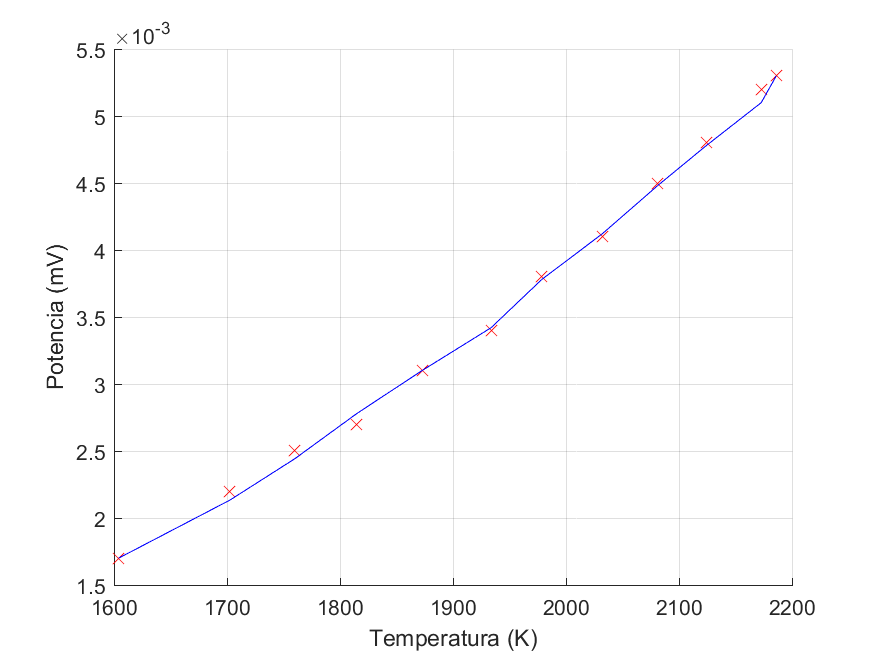
\includegraphics[width=0.8\textwidth]{assets/Stefan_Boltzmann1.png}
\caption{\label{fig:sb1}Potencia emitida en función de la temperatura.}
\end{figure}

En base a lo anterior podemos empezar a inferir el grado del polinomio: De grado 1 sabemos que no es porque si así lo fuera los coeficientes serían casi iguales, probemos con 2: $1.36^2 = 1.85$, con 3: $1.36^3 = 2.52$, y con 4: $1.36^4 = 3.42$. Lo que nos lleva a inferir que el grado del polinomio debería ser estar entre 3 y 4 (más cerca de 4).

Para calcular el grado del polinomio podemos utilizar el \href{https://en.wikipedia.org/wiki/Pearson_correlation_coefficient}{coeficiente de correlación Pearson}\footnote{Ver la letra de la práctica}, el cual en MATLAB está disponible a través de la función \href{https://www.mathworks.com/help/matlab/ref/corrcoef.html}{corrcoef}. El codigo que calcula el grado del polinomio es el siguiente:
\\
\lstinputlisting{assets/calcular_grado.m}

Acá nos topamos con un gran problema, según el coeficiente de Pearson, el grado que mejor ajusta es 3!

Pero según nuestro background teórico el grado debe ser 4 y, además, nuestra deducción anterior sujiere que el grado del polinomio está más cerca de 4 que de 3. Más adelante especularemos sobre este tema, por ahora tratemos de encontrar el grado del polinomio, para eso utilizaremos la función \href{https://www.mathworks.com/help/matlab/ref/polyfit.html}{polyfit} de MATLAB, la cual implementa el algoritmo de aproximación por mínimos cuadrados.

Un resultado interesante aparece cuando combinamos $polyfit$ con el logaritmo natural, por qué?

Se supone que tenemos la relación $V_s = \omega T^n$, para algún $\omega$ y algún $n$, entonces, si aplicamos logaritmos en ambos lados de la la igualdad tenemos:

\begin{align*}
    \log(V_s) &= \log(\omega T^n) \Rightarrow\\
    \log(V_s) &= \log(\omega) + n\log(T) \Rightarrow\\
    y &= nx + b & y = V_s, b = \log(\omega), x = \log(T)
\end{align*}

Lo que permite calcular el grado $n$ del polinomio y su coeficiente principal $e^\omega$\footnote{$y = \log_b(x) \Rightarrow x = b^y$}.

Este método nos da como resultado $n = 3.61$ y $\omega = e^{-33} = 4.6190 \times 10^{-15}$.

Vemos que el exponente está más cerca de 4 que de 3, sin embargo, el error es extremadamente grande. Hay varios factores que contribuyeron a este error:

\begin{itemize}
    \item Errores de medicón afectados por la presición de los instrumentos
    \item Errores de medición debidos a potencial falta de rigurosidad para con el procedimiento
    \item Error al determinar la distancia a la que debía estar el sensor de la lámpara
\end{itemize}

La figura \ref{fig:sb2} muestra dos gráficas supuerpuestas. Por un lado, la potencia emitida en función de la temperatura a la cuarta potencia, y por otro lado la recta de ajuste calculada por mínimos cuadrados.

\begin{figure}[h!]
\centering
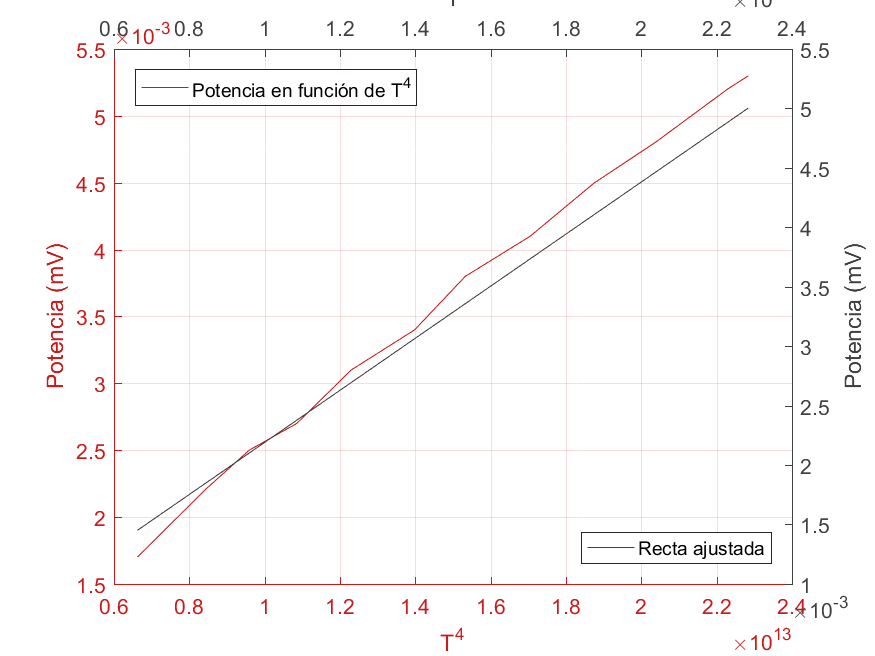
\includegraphics[width=0.8\textwidth]{assets/Stefan_Boltzmann2.png}
\caption{\label{fig:sb2}Potencia en función de $T^4$ y recta ajustada.}
\end{figure}

En la letra de la práctica se pregunta sobre la \textbf{pendiente de dicha recta} ($\omega = 2.1908 \times 10^{-16}$). En párrafos previos ya nos hemos referido a dicha pendiente, pero con otro nombre: \textit{coeficiente director del polinomio}.

Entonces, la pendiente de la gráfica representa el factor de cambio del valor de la radiación respecto a la variación de la cuarta potencia de la temperatura, también se podría decir que es la derivada\newpage de dicha función. En nuestro caso, nos interesa el siguiente resultado:
% Force un newpage para que me quede bien mas abajo
Basados en el supuesto de que la radiación medida con el sensor es una fracción de la energía E emitida por el cuerpo negro, llegamos a la siguiente formula:

\begin{align}
\exists k \in R / E = k V_s
\end{align}

%\newpage % Solo para poder rellenar un poco mas la hoja siguiente
Es decir, la radiación emitida $V_s$ el una fracción de la potencia (mayor o menor dependerá del k). Si aplicamos esto sobre la ecuación \ref{eq:SB}, nos da que la pendiente $\omega$ de la gráfica es efectivamente igual a $\frac{\sigma}{k}$!. Lo que nos permite deducir lo siguiente:

\begin{align*}
E &= \sigma T^4 & y\\
V_s &= \omega T^4 & \Rightarrow\\
kV_s &= \sigma T^4 & \Rightarrow\\
k &= \frac{\sigma}{\omega} & y\\
E &= wkT^4
\end{align*}

Este resultado permite entonces calcular k y, consecuentemente, calcular E.

En el apéndice \ref{appendix:sb} se puede ver el código Matlab utilizado para realizar los cálculos.

\newpage
\section{Ley de desplazamiento de Wien}

Este esperimento es un poco mas sencillo que el anterior. Consiste en determinar la longitud de onda a la que se obtiene la mayor intensidad de radiación. Para ejecutar el mismo utilizamos un simulador desarrollado por el Prof. Salvador Hurtado Fernández\footnote{Ver letra de la práctica}.

\subsection{Procedimiento}

Para iniciar el experimento ingresamos al sitio http://labovirtual.blogspot.com.uy/2009/07/radiacion-del-cuepo-negro\_11.html, habilitamos Flash, y procedemos de la siguiente manera:

\begin{enumerate}
    \item Seleccionar la temperatura en el Control de Temperatura e iniciar el calentamiento con
el pulsador rojo. Esperar mientras se analiza la radiación emitida y se dibuja la curva.
    \item Determinar la longitud de onda a la que se obtiene la mayor intensidad de radiación.
    \item Repetir el procedimiento para 20 temperaturas diferentes.
\end{enumerate}

Los datos obtenidos del simulador se pueden observar en la tabla \ref{tabla2}, como se puede observar, se tomaron 25 muestras en vez de 20.

\begin{table}[h!]
\centering
\begin{tabular}{c|c}
Temperatura ($K$) & Longitud de onda màxima $\lambda_{max}$ ($nm$)\\\hline
3800 & 762 \\
3968 & 730 \\
4071 & 712 \\
4092 & 708 \\
4185 & 692 \\
4196 & 690 \\
4383 & 661 \\
4393 & 659 \\
4425 & 655 \\
4508 & 643 \\
4590 & 631 \\
4603 & 629 \\
4716 & 614 \\
4779 & 606 \\
4913 & 590 \\
4945 & 586 \\
5007 & 579 \\
5092 & 569 \\
5180 & 559 \\
5227 & 554 \\
5300 & 547 \\
5498 & 527 \\
5519 & 525 \\
5643 & 513 \\
5685 & 510
\end{tabular}
\caption{\label{tabla2}Wien}
\end{table}

\subsection{Exposición de resultados y análisis}

En los datos se observa que a medida que aumenta la temperatura, disminuye $\lambda_{max}$, además, se observa que la relación es lineal ($\frac{5685}{3800} \approx \frac{762}{510}$).

La figura \ref{fig:wien1} muestra la longitud de onda en función del inverso de la temperatura, al observar dicha gráfica la linealidad se hace evidente.

Entonces: A mayor temperatura, menor longitud de onda, cuanto menor es la longitud de onda, mayor es la energía de la misma.

\begin{figure}[h!]
\centering
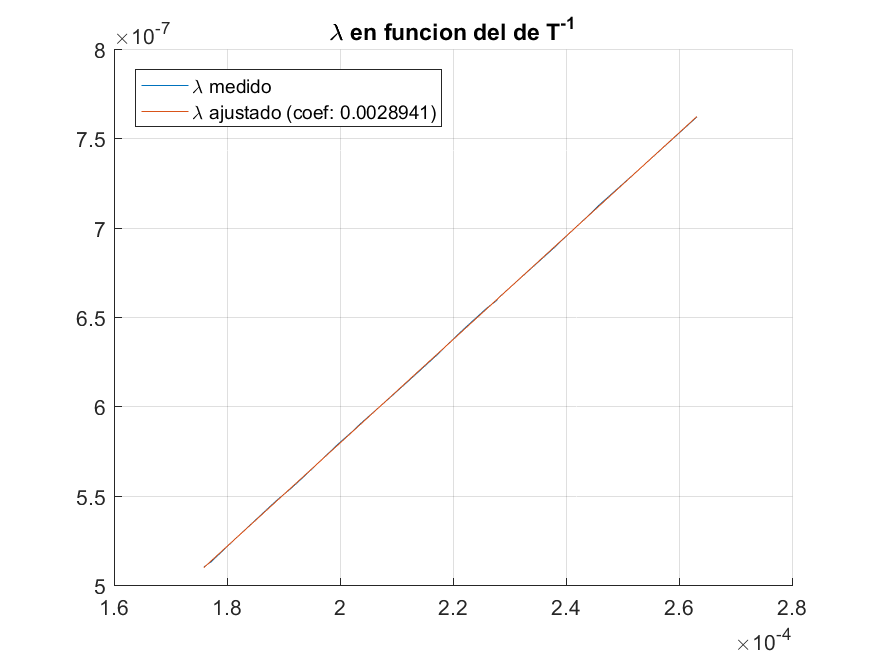
\includegraphics[width=0.8\textwidth]{assets/Wien.png}
\caption{\label{fig:wien1}.}
\end{figure}

Aproximando por mínimos cuadrados tenemos que se logra una recta con una pendiente igual a $2.8941 \times 10^{-3}$, muy parecido al la constante de Wien (esto solo demuestra la fidelidad del simulador).

En la introducción comentabamos que el sol tiene una temperatura media de 5800K. Aplicando la ley de Wien tenemos que la logitud de onda máxima $\lambda_{max}$ se sitúa en los 500nm (ver ecuaciones \ref{eq:Wien} y \ref{eq:WienSun}).

Estas longitudes de onda se sitúan en la región verde del espectro de la luz visible, pero el Sol irradia continuamente fotones con longitudes de onda más largas y más cortas que $\lambda_{max}$ y por eso el ojo humano percibe el color del Sol como blanco-amarillo.

En el apéndice \ref{appendix:wien} se puede ver el código Matlab utilizado para realizar los cálculos.

\newpage
\begin{appendices}

\section{Script Stefan\_Boltzmann.m}
\label{appendix:sb}

Script utilizado para el experimento N° 1.

\lstinputlisting{assets/stefan_boltzmann.m}

\newpage
\section{Script Wien.m}
\label{appendix:wien}

Script utilizado para el experimento N° 2.

\lstinputlisting{assets/wien.m}

\end{appendices}

\begin{thebibliography}{9}
\bibitem{practica2}
  Instituto de Física - Facultad de Ciencias,
  \emph{Letra de la práctica 2 - Introducción a las Ciencias de la Tierra y el Espacio I},
  Online at https://eva.udelar.edu.uy/mod/resource/view.php?id=408135
\bibitem{radiationManual}
  PASCO Scientific,
  \emph{Thermal radiation system manual},
  Oline at https://eva.udelar.edu.uy/pluginfile.php/911292/mod\_folder/content/0/Thermal-Radiation-System-Manual-TD-8553.pdf
\bibitem{fundamentosSimulador}
  I.E.S. Aguilar y Cano,
  \emph{Fundamentos teoricos básicos},
  Online at http://www.juntadeandalucia.es/averroes/centros-tic/41008970/helvia/sitio/upload/1La\_fisica\_del\_siglo\_XX.pdf
\end{thebibliography}

\end{document}
